\documentclass[10pt]{article}

\usepackage{akteach}
\usepackage{amsmath}
\usepackage{amsfonts}
\usepackage{amssymb}
\usepackage{amsthm}
\usepackage{float}
\usepackage{algpseudocode}
\usepackage[all]{xy}

\usepackage{listings}
\usepackage{color}

\definecolor{dkgreen}{rgb}{0,0.6,0}
\definecolor{gray}{rgb}{0.5,0.5,0.5}
\definecolor{mauve}{rgb}{0.58,0,0.82}

\lstset{
  language=Python,
  aboveskip=3mm,
  belowskip=3mm,
  showstringspaces=false,
  columns=flexible,
  basicstyle={\small\ttfamily},
  numbers=none,
  numberstyle=\tiny\color{gray},
  keywordstyle=\color{blue},
  commentstyle=\color{dkgreen},
  stringstyle=\color{mauve},
  breaklines=true,
  breakatwhitespace=true,
  tabsize=3
}


\newcommand{\C}{\mathbb{C}}
\newcommand{\Q}{\mathbb{Q}}
\newcommand{\K}{\mathbb{K}}
\newcommand{\proj}{\mathbb{P}}
\newcommand{\T}{\mathbb{T}}
\newcommand{\F}{\mathbb{F}}
\newcommand{\Z}{\mathbb{Z}}
\newcommand{\N}{\mathbb{N}}
\newcommand{\cp}{\mathbb{C}P}
\newcommand{\A}{\mathcal{A}}
\newcommand{\BB}{\mathcal{B}}
\newcommand{\CC}{\mathcal{C}}
\newcommand{\NN}{\mathcal{N}}
\newcommand{\MM}{\mathcal{M}}
\newcommand{\E}{\mathcal{E}}
\newcommand{\FF}{\mathcal{F}}
\newcommand{\G}{\mathcal{G}}
\newcommand{\eps}{\varepsilon}
\newcommand{\Hom}{\text{Hom}}
\newcommand{\Div}{\text{div}}
\newcommand{\Res}{\text{Res}}
\newcommand{\ord}{\text{ord}}
\newcommand{\Deg}{\text{deg}}
\newcommand{\mult}{\text{mult}}

\newcommand{\id}{\text{id}}
\newcommand{\Tr}{\text{Tr}}
\newcommand{\ad}{\text{ad}}
\newcommand{\Ad}{\text{Ad}}
\newcommand{\Aut}{\text{Aut}}
\newcommand{\der}{\text{der}}
\newcommand{\GL}{\text{GL}}
\newcommand{\gl}{\mathfrak{gl}}
\newcommand{\rad}{\mathfrak{rad}}
\newcommand{\inhook}{\hookrightarrow}
\newcommand{\sgn}{\text{sign}}

\begin{document}

\akteachheader{Numerical Analysis (CS 450)}%
{Homework Set 6, Bill Karr}

\akteachprobhead{%
  Problem 1: Numerical Methods for ODEs and Dissipation (20 points)
}

\begin{itemize}

\item[(a)] Let $ v = u' \Rightarrow v' = u'' = - u $. Thus we have \begin{align*}
u' &=  v, \quad u(0) = 1 \\
v' &= - u, \quad v(0) = 0.
\end{align*} The exact solution is $ u(t) = \cos(t) $.

\item[(b)] See \verb+ode.py+.

\begin{itemize}

\item[(i)] For 4th order Runge-Kutta, I have the following code. \begin{lstlisting}
def runge_kutta(f, h, t0, tf, v0):
    n = int((tf - t0) / h) + 1
    v = np.zeros((n, 2))
    v[0] = v0
    t = np.linspace(t0, tf, n)
    for k in xrange(n - 1):
        k1 = f(v[k])
        k2 = f(v[k] + (h / 2) * k1)
        k3 = f(v[k] + (h / 2) * k2)
        k4 = f(v[k] + h * k3)
        v[k + 1] = v[k] + h * (k1 + 2 * k2 + 2 * k3 + k4) / 6
    return v.T, t
\end{lstlisting}

\item[(ii)] For the leapfrog method, I have the following code. \begin{lstlisting} 
def leapfrog(f, h, t0, tf, v0):
    n = int((tf - t0) / h) + 1
    v = np.zeros((n, 2))
    v[0] = v0
    t = np.linspace(t0, tf, n)
    v[1] = v[0] + h * f(v[0])
    v[1] = v[0] + (h / 2) * (f(v[0]) + f(v[1]))
    for k in xrange(n - 2):
        v[k + 2] = v[k] + 2 * h * f(v[k + 1])
    return v.T, t
\end{lstlisting}

\end{itemize} Using the maximum norm to compute errors against the exact solution over the first period, I obtain an empirical order of convergence of 4 and 2 for the two methods respectively. See my data below. \begin{verbatim}
Runge-Kutta

For h = 0.785398, max error = 0.0171143
For h = 0.392699, max error = 0.00100789, EOC = 4.08579
For h = 0.19635, max error = 6.15575e-05, EOC = 4.03327
For h = 0.0981748, max error = 3.78832e-06, EOC = 4.0223
For h = 0.0490874, max error = 2.34872e-07, EOC = 4.01161
For h = 0.0245437, max error = 1.46194e-08, EOC = 4.00592
For h = 0.0122718, max error = 9.11817e-10, EOC = 4.00299
For h = 0.00613592, max error = 5.69285e-11, EOC = 4.00152
For h = 0.00306796, max error = 3.55607e-12, EOC = 4.0008

Leapfrog

For h = 0.785398, max error = 0.650047
For h = 0.392699, max error = 0.130017, EOC = 2.32184
For h = 0.19635, max error = 0.0314223, EOC = 2.04884
For h = 0.0981748, max error = 0.00776133, EOC = 2.01742
For h = 0.0490874, max error = 0.00193517, EOC = 2.00385
For h = 0.0245437, max error = 0.000483469, EOC = 2.00096
For h = 0.0122718, max error = 0.000120847, EOC = 2.00024
For h = 0.00613592, max error = 3.02108e-05, EOC = 2.00005
For h = 0.00306796, max error = 7.55263e-06, EOC = 2.00002
\end{verbatim} 

Below, I show the 300th to 309th periods of the two approximate solutions.

\begin{figure}[H]
  \centering
    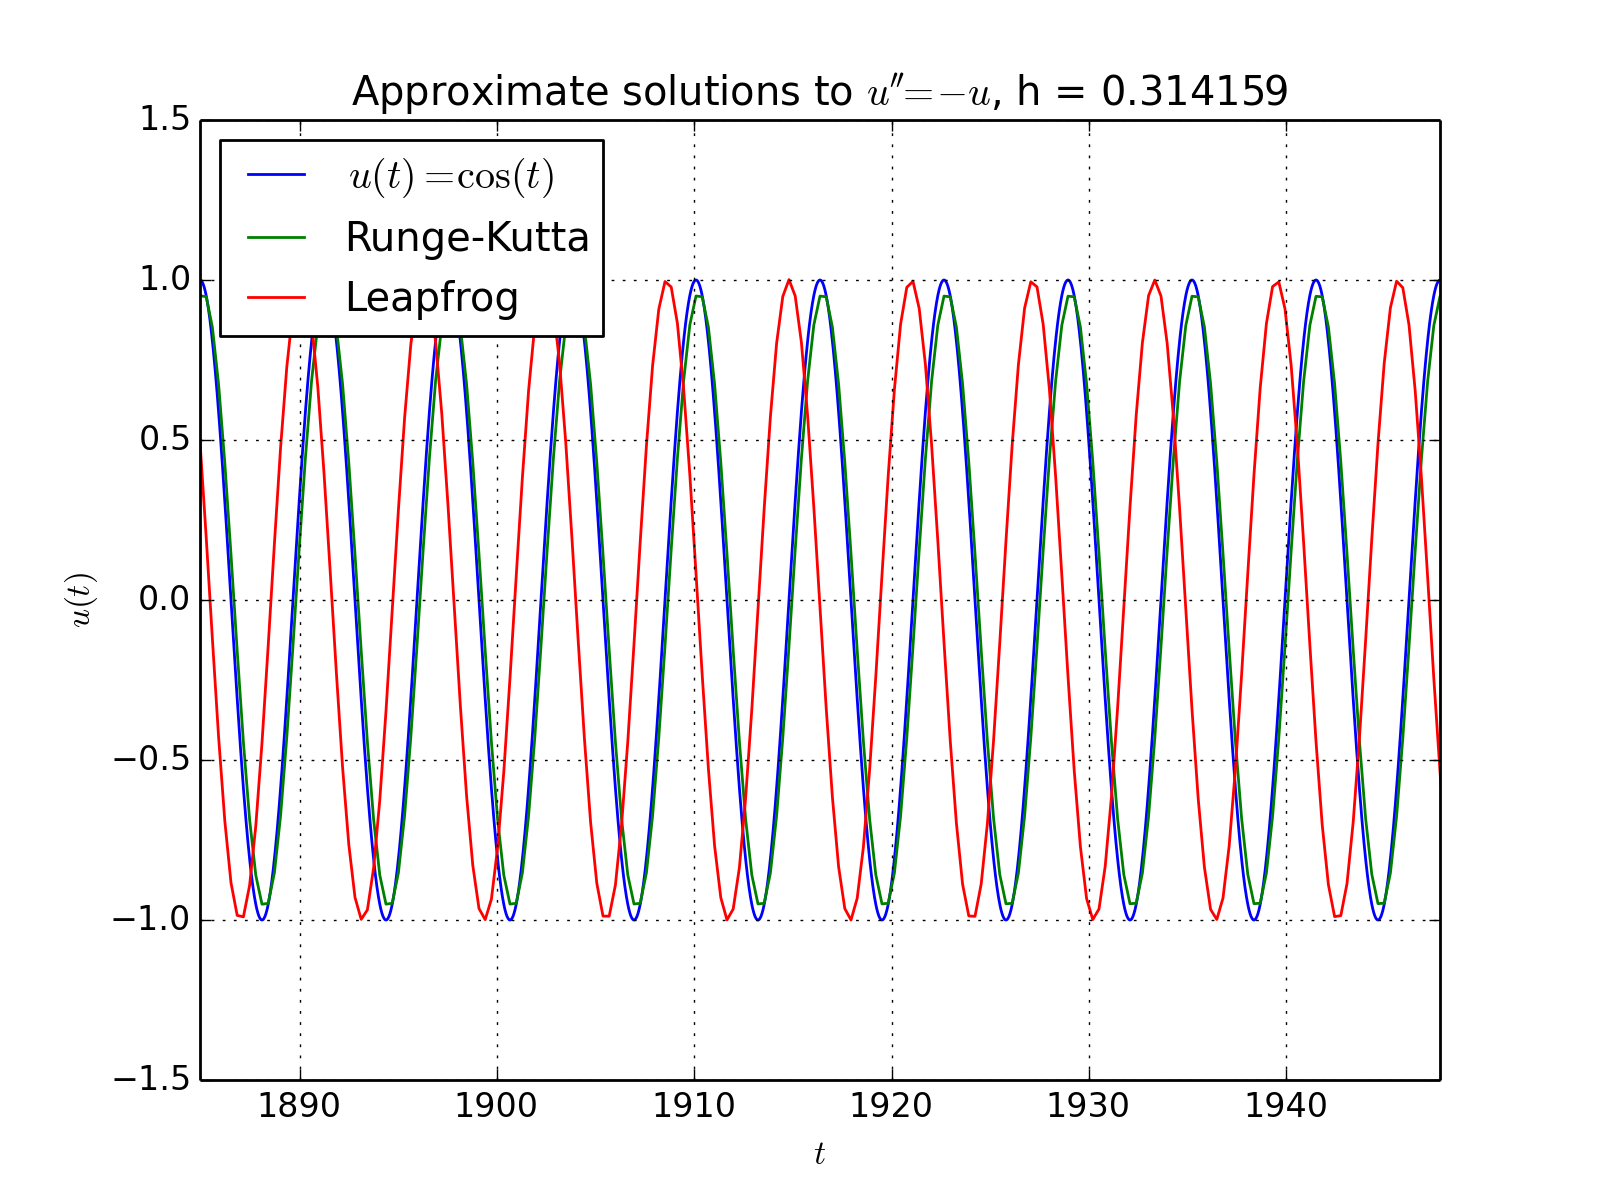
\includegraphics[scale=0.6]{ode}
\end{figure}

\item[(c)] See \verb+ode.py+ for my code. The following are plots of the energy of my approximate solutions. Even though Runge-Kutta converges faster, we see energy dissipating over time, whereas the leapfrog method seems to conserve energy. In orbital dynamics, energy dissipating is problematic since it means that a periodic system will have bad approximations after long periods of time. Using a dissipative method for a satellite would mean the satellite would lose energy over time. In other words it would either slow down or get closer to Earth over long periods of time.

\begin{figure}[H]
  \centering
    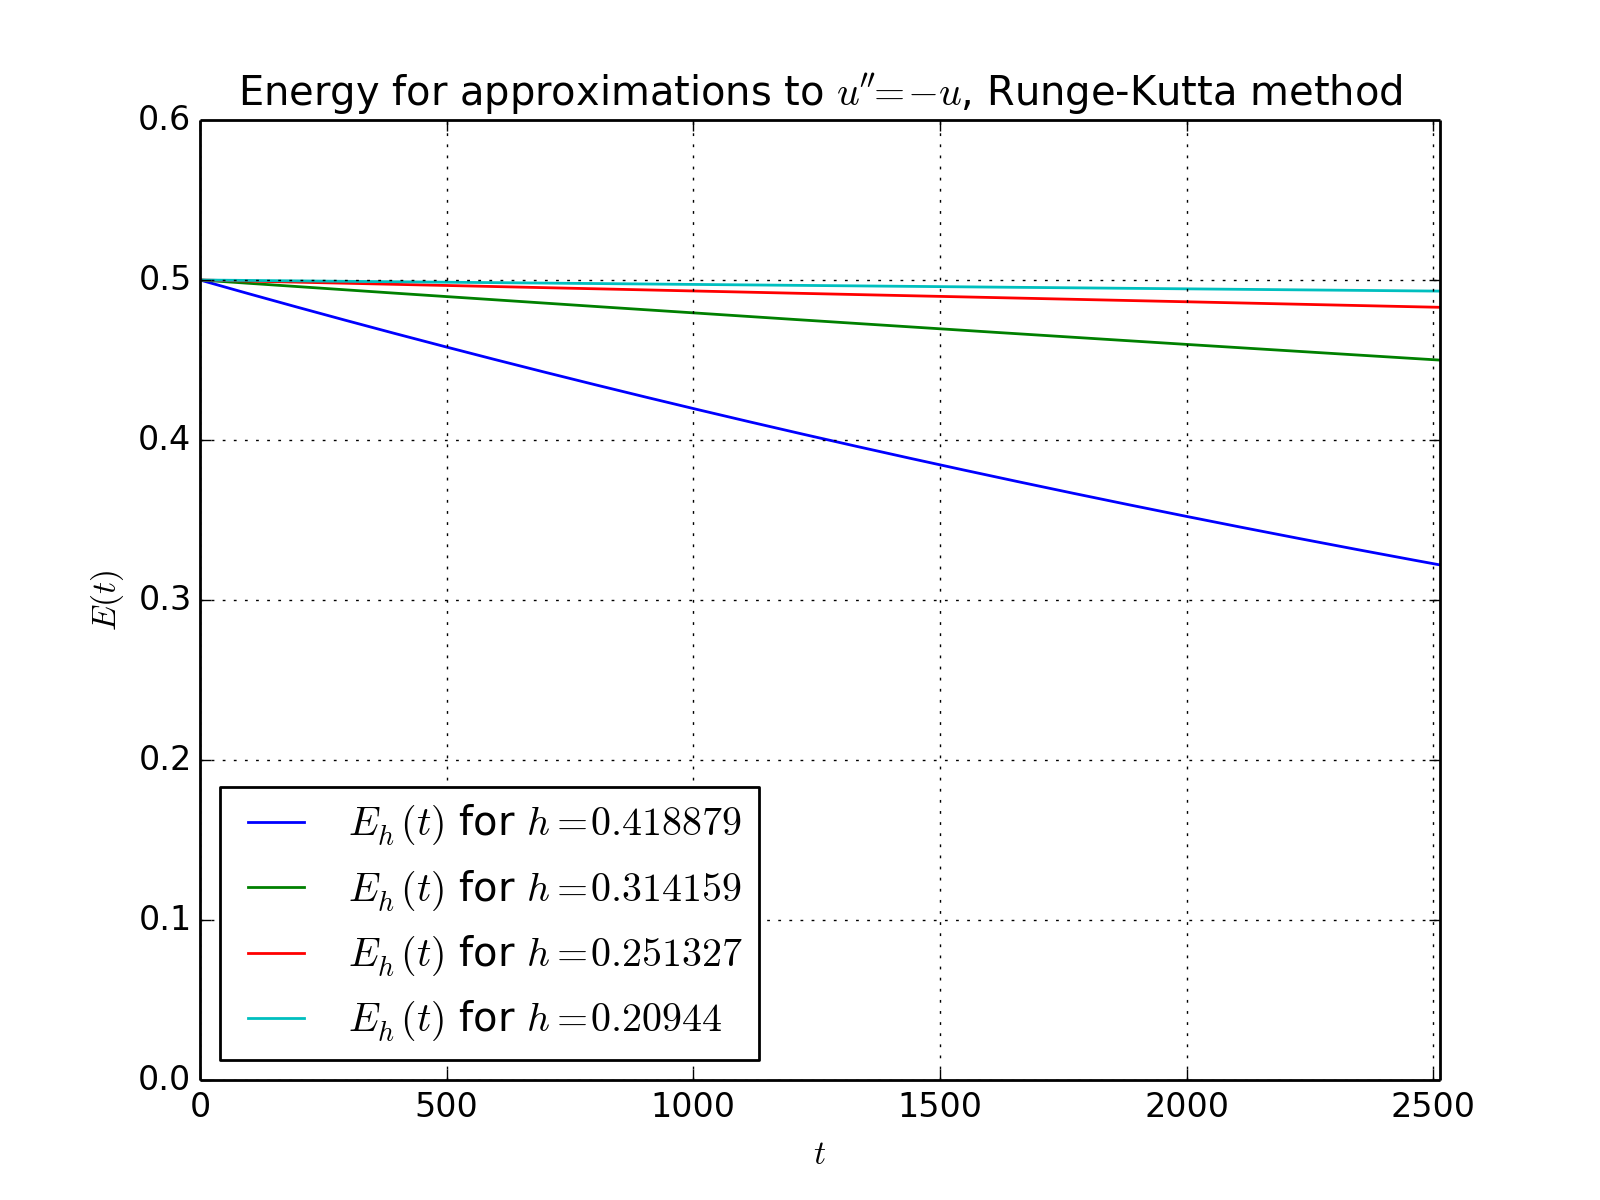
\includegraphics[scale=0.6]{energy_runge-kutta}
\end{figure}

\begin{figure}[H]
  \centering
    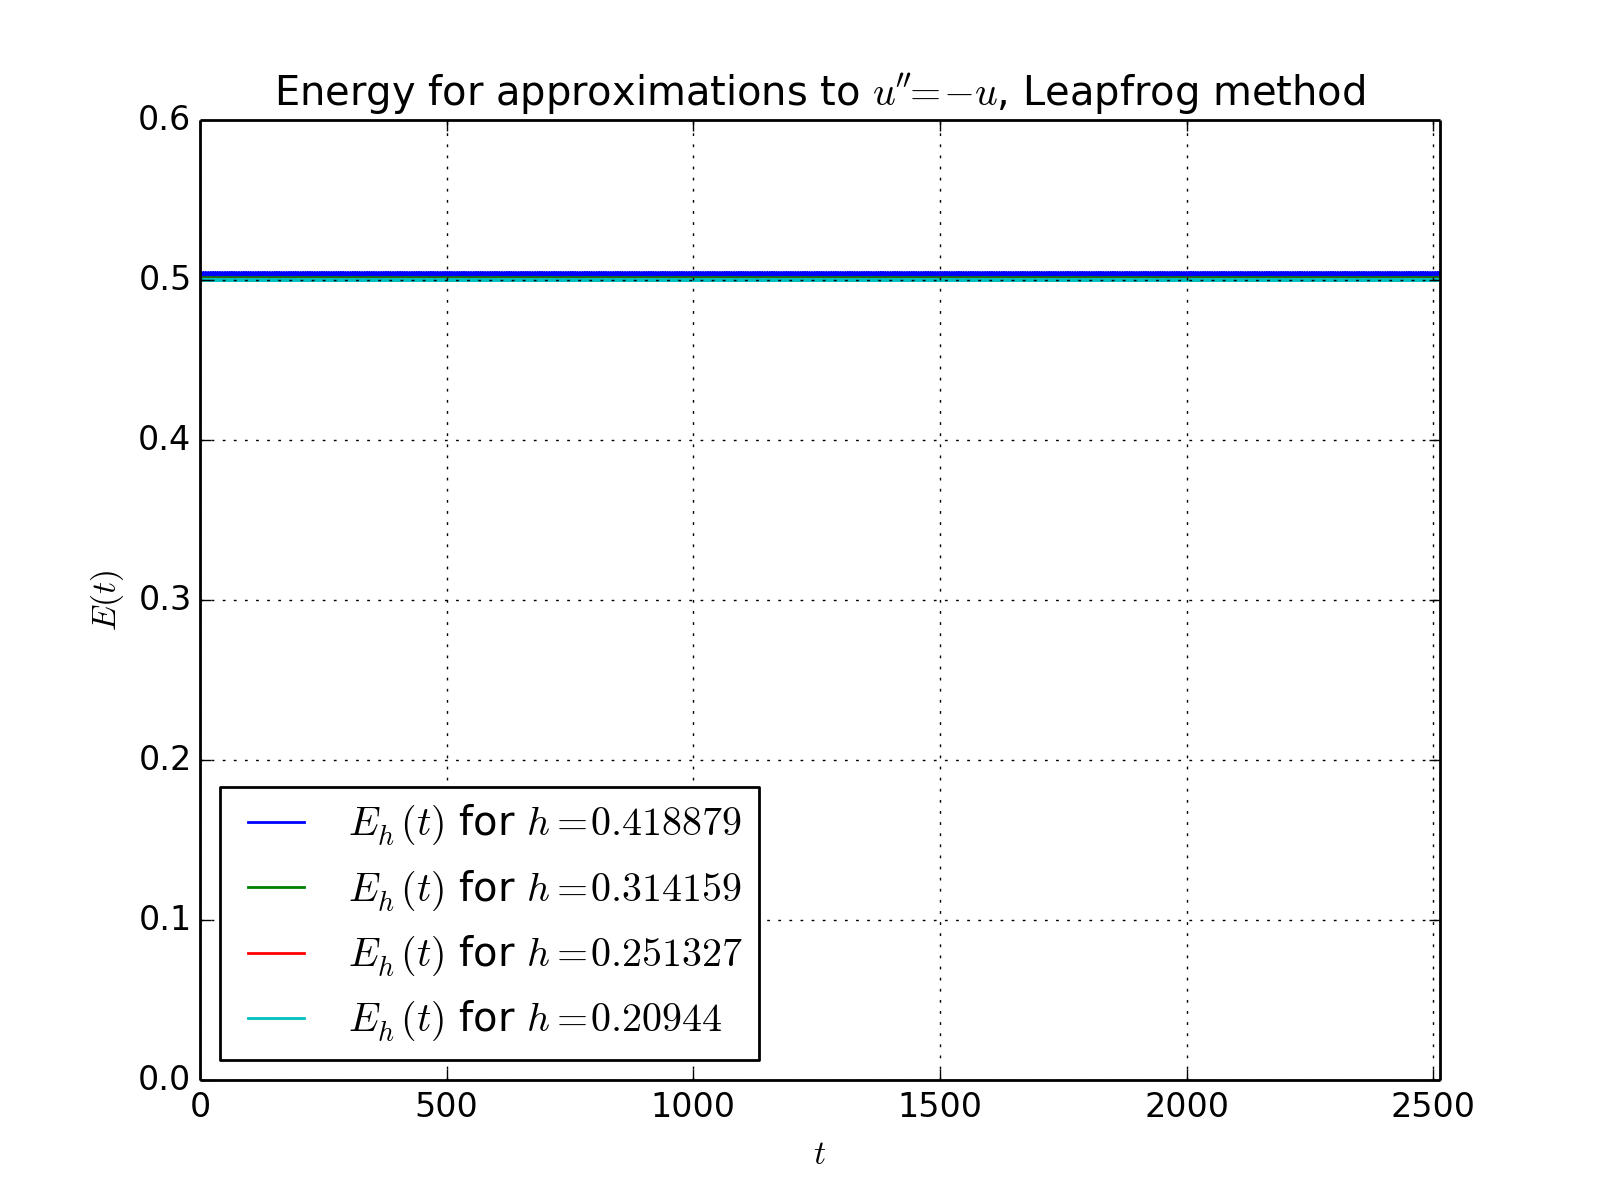
\includegraphics[scale=0.6]{energy_leapfrog}
\end{figure}

\end{itemize}

\newpage

\akteachprobhead{%
  Problem 2: BVP theory (20 points)
}

Consider the two-point BVP for the second-order ODE $$
u'' = u, 0 < t < b
$$ with boundary conditions $ u(0) = \alpha, u(b) = \beta $. 

\begin{itemize}

\item[(a)] If we let $ v = u' $, then we obtain \begin{align*}
\begin{bmatrix}
u \\
v
\end{bmatrix} ' = \begin{bmatrix}
0 & 1 \\
1 & 0
\end{bmatrix} \begin{bmatrix}
u \\
v
\end{bmatrix}
\end{align*} with boundary conditions \begin{align*}
\begin{bmatrix}
1 & 0 \\
0 & 0
\end{bmatrix} \begin{bmatrix}
u(\alpha) \\
v(\alpha)
\end{bmatrix} + \begin{bmatrix}
0 & 0 \\
1 & 0
\end{bmatrix} \begin{bmatrix}
u(\beta) \\
v(\beta)
\end{bmatrix} = \begin{bmatrix}
\alpha \\
\beta
\end{bmatrix}.
\end{align*} 

\item[(b)] Notice that $ u = e^{\pm t}, v = e^{\mp t} $ forms a pair of independent solutions. If we find the fundamental sotuions using these, we obtain \begin{align*}
\begin{bmatrix}
\frac{e^t + e^{-t}}{2} & \frac{e^t - e^{-t}}{2} \\
\frac{e^t - e^{-t}}{2} & \frac{e^t + e^{-t}}{2}
\end{bmatrix} = \begin{bmatrix}
\cosh(t) & \sinh(t) \\
\sinh(t) & \cosh(t)
\end{bmatrix}.
\end{align*}

\item[(c)] The matrix of the system has eigenvalues $ \pm 1$. Since one of them has positive real part, the solutions are not stable.

\item[(d)]$$Q = \begin{bmatrix}
1 & 0 \\
0 & 0
\end{bmatrix} \begin{bmatrix}
1 & 0 \\
0 & 1
\end{bmatrix} + \begin{bmatrix}
0 & 0 \\
1 & 0
\end{bmatrix} \begin{bmatrix}
\cosh(b) & \sinh(b) \\
\sinh(b) & \cosh(b)
\end{bmatrix} = \begin{bmatrix}
1 & 0 \\
\cosh(b) & \sinh(b)
\end{bmatrix} $$

\item[(e)] The rescaled solution is $$
\Phi(t) = \begin{bmatrix}
\cosh(t) & \sinh(t) \\
\sinh(t) & \cosh(t)
\end{bmatrix} \begin{bmatrix}
1 & 0 \\
-\frac{ \cosh(b)}{\sinh(b)} & \frac{1}{\sinh(b)}  \end{bmatrix} = \begin{bmatrix}
\cosh(t) - \sinh(t) \frac{\cosh(b)}{\sinh(b)} & \frac{\sinh(t)}{\sinh(b)} \\
\sinh(t) - \cosh(t)  \frac{\cosh(b)}{\sinh(b)} & \frac{\cosh(t)}{\sinh(b)} 
\end{bmatrix}
$$

\item[(f)] The eigenvalues of $Q$ are $ 1$ and $ \sinh(b) $. As $ b \to 0 $, $ \sinh(b) \to \infty $ and thus, the conditioning number is $ \sinh(b) /1 \to \infty $ as $ b \to \infty $ and it grows exponentially with $b$.

\end{itemize}

\newpage

\akteachprobhead{%
  Problem 3: BVPs and the method of manufactured solutions (20 points)
}

\begin{itemize}

\item[(a)] See \verb+bvp.py+ for my code. Here is my function:  \begin{lstlisting} 
def bvp_solve(p, q, f, x, u_a, u_b):
    n, dx = len(x), x[1] - x[0]
    
    D2 = sps.diags([1, -2, 1] / dx ** 2, offsets=[0, 1, 2], shape=(n - 2, n))
    D1 = sps.diags([-1, 1] / (2 * dx), offsets=[0, 2], shape=(n - 2, n))
    D0 = sps.diags([1], offsets=[1], shape=(n - 2, n))
    
    P = sps.diags([p(x[1:-1])], [0])
    Q = sps.diags([q(x[1:-1])], [0])
    
    left_bv = sps.diags([1], offsets=[0], shape=(1,n))
    right_bv = sps.diags([1], offsets=[n-1], shape=(1,n))
    
    A = sps.csr_matrix(sps.vstack([left_bv, D2 + P * D1 + Q * D0, right_bv]))
    b = f(x)
    b[0], b[-1] = u_a, u_b
    
    return sla.spsolve(A, b)
\end{lstlisting}

\item[(b)] See \verb+bvp.py+ for my code.

\item[(c)] Below is my plot showing the error results for each of the three cases compared to the line given by second order convergence. The error does not decrease monotonically once $h$ reaches $ h \approx 10^{-4.5} $, at which point the error begins get worse. This could be because of poor conditioning of the matrix $A$ in the BVP solver for small values of $h$.

\begin{figure}[H]
  \centering
    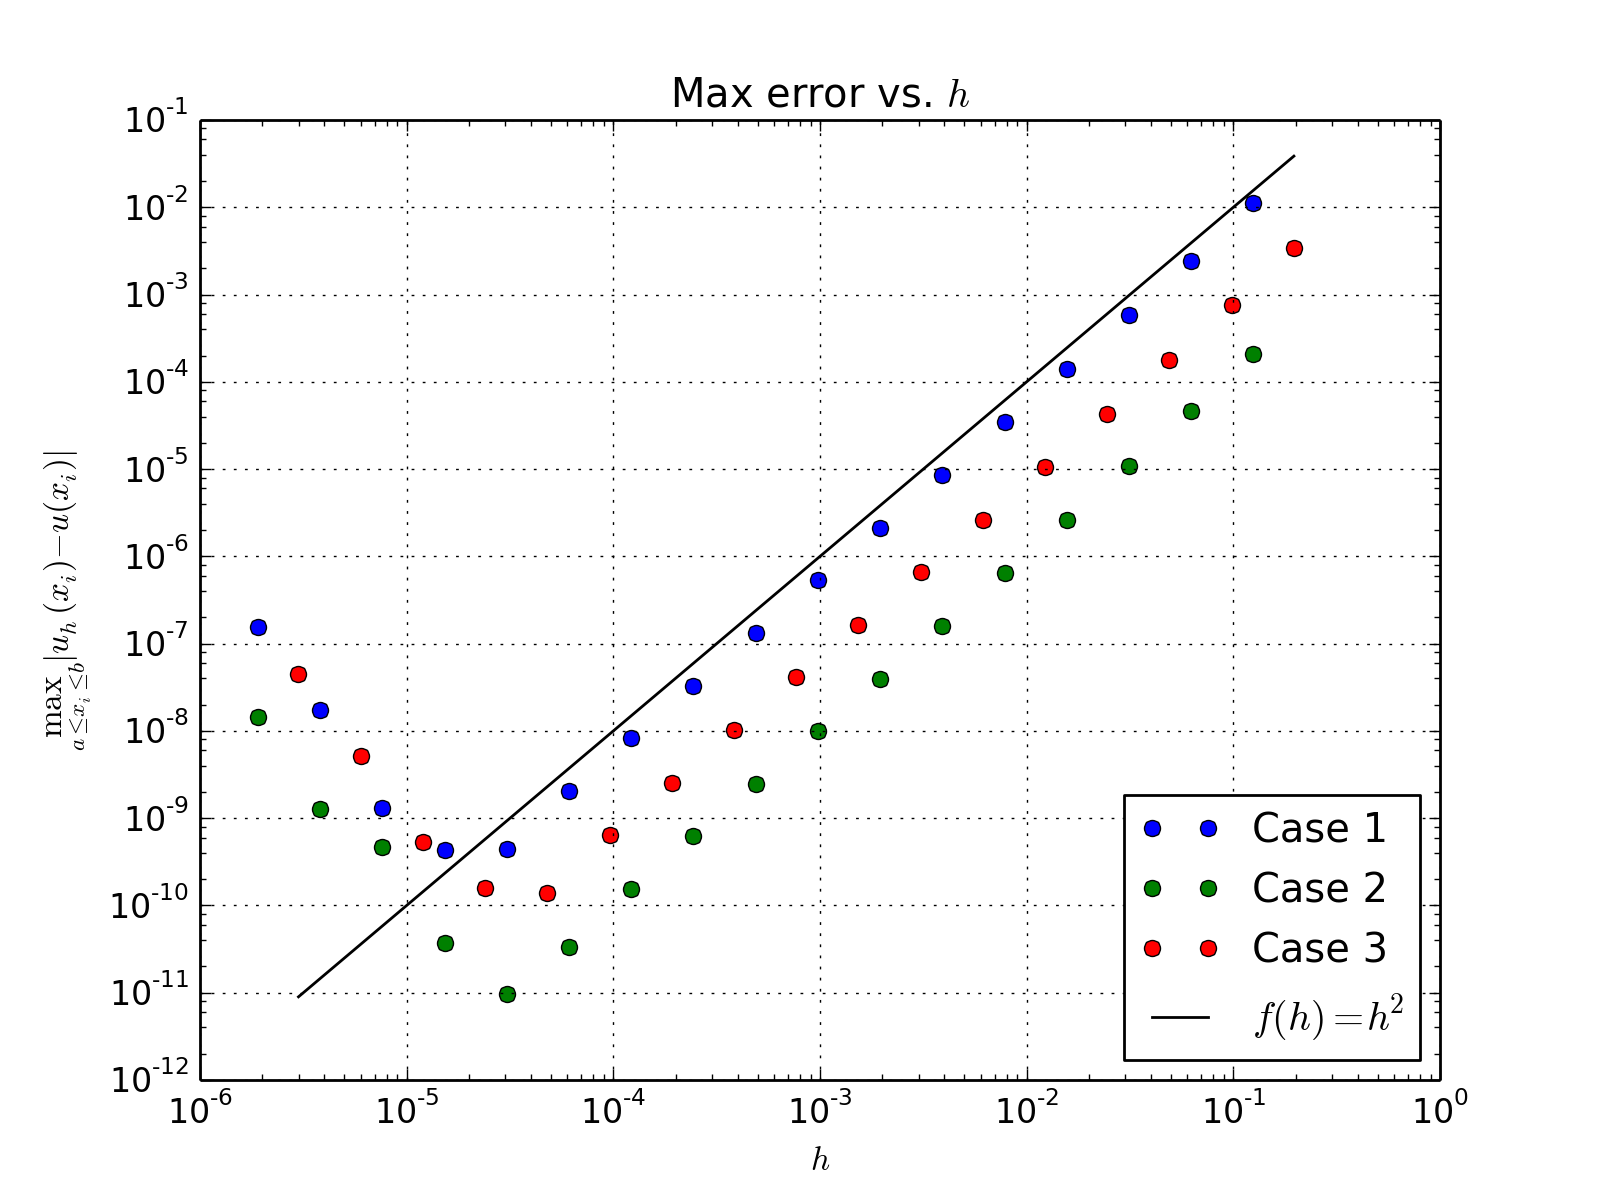
\includegraphics[scale=0.6]{errors}
\end{figure}

\item[(d)] Below is my plot showing the conditioning numbers of the matrices $A$ vs. the size of $A$ for $ n = 2^k, k = 3, ... , 10 $. If we extrapolate, we see that as $k$ becomes larger, the conditioning number will reach $ 10^{15} $ which is approximately $1/ \eps_{\text{mach}}$, so poor conditioning is likely the cause of the increased error for small $h$ in the previous part.

\begin{figure}[H]
  \centering
    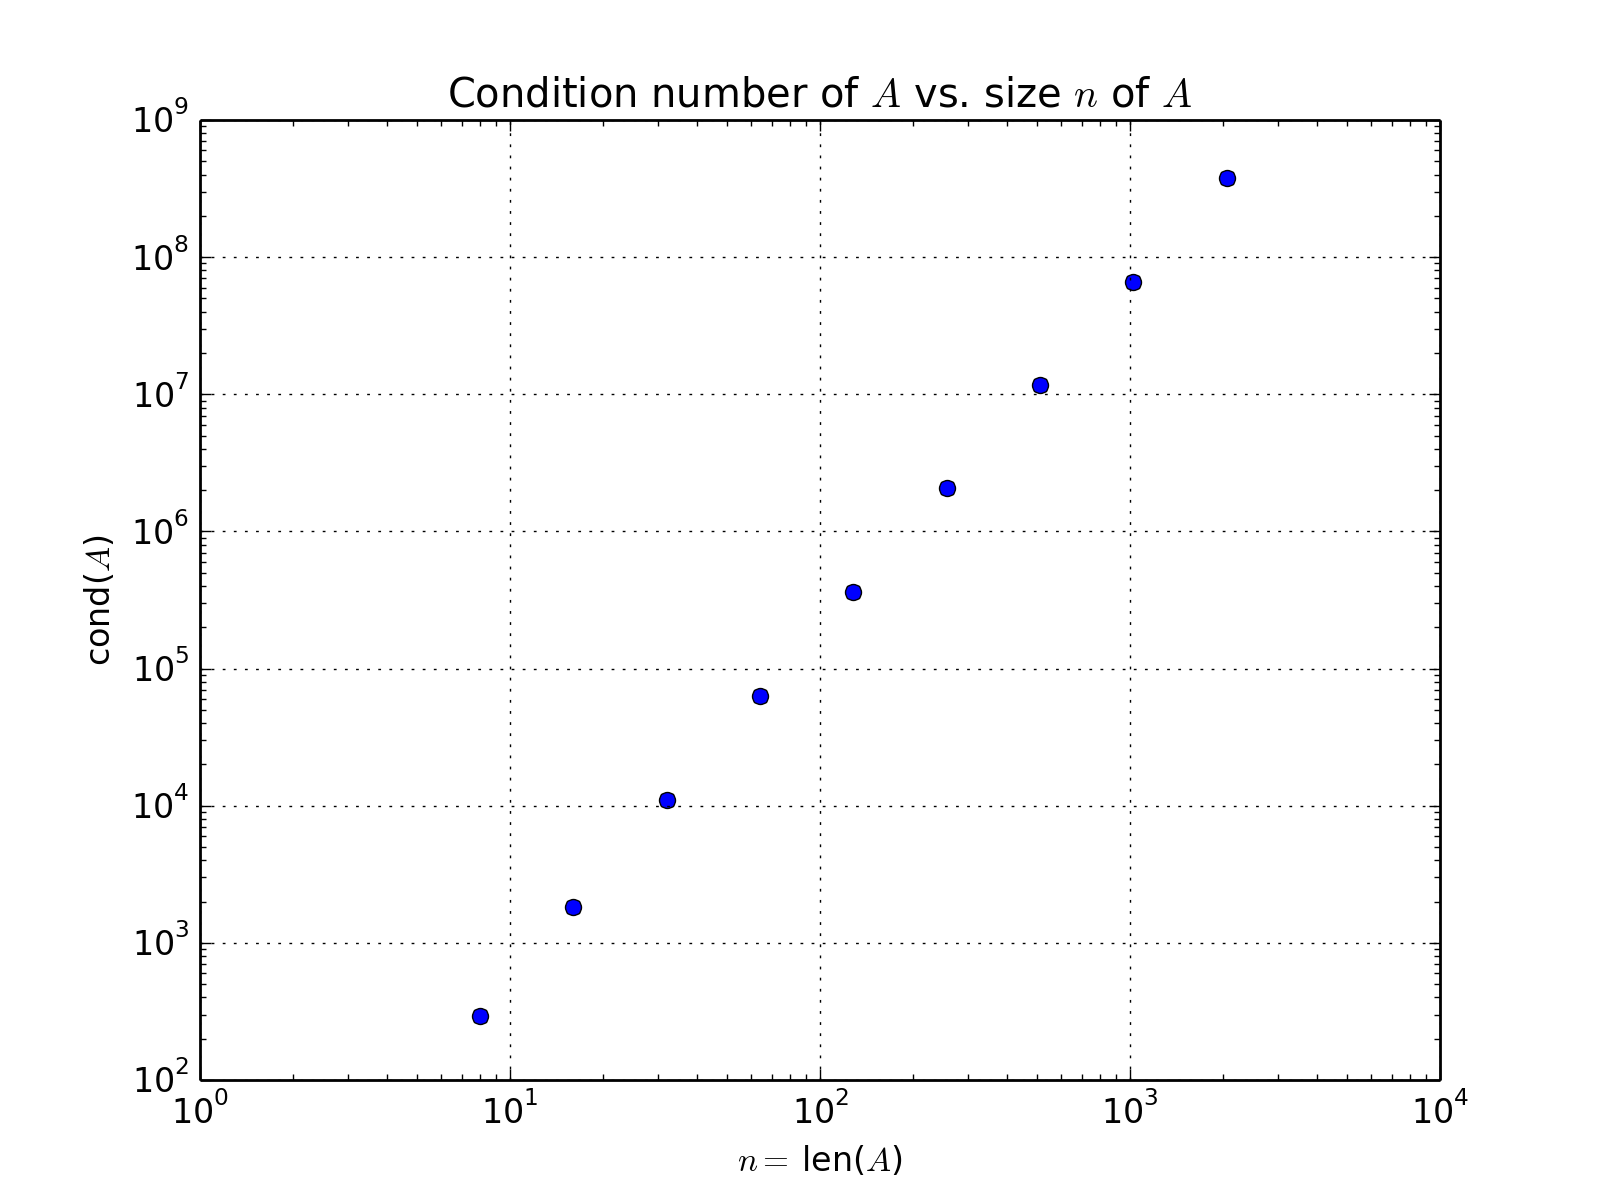
\includegraphics[scale=0.6]{conds}
\end{figure}

\end{itemize}

\newpage

\akteachprobhead{%
  Problem 4: Iterative methods (20 points)
}

\begin{itemize}

\item[(a)] Prove that the Successive Over-Relaxation method diverges if $ \omega \not\in (0,2) $.

\begin{proof} Let $ L $ and $U$ be the lower triangular and strictly upper triangular parts of $A$, respectively. The Gauss-Seidel method can be rewritten as $$
\mathbf{x}^{(k+1)} = L^{-1} ( \mathbf{b} - U \mathbf{x}^{(k)} ).
$$ and the Successive Over-Relaxation method can be written as $$
\mathbf{x}^{(k+1)} = (1 - \omega) \mathbf{x}^{(k)} + \omega L^{-1} ( \mathbf{b} - U \mathbf{x}^{(k)} ).
$$ Suppose $ \omega \not\in (0,2) $ and assume $ \mathbf{x}^{(k)} $ converges to some vector $ \mathbf{x} $ as $ k \to \infty $. Then, we can take the limit of the above equation and obtain $$
\mathbf{x} = (1 - \omega)\mathbf{x} + \omega L^{-1}( \mathbf{b} - U \mathbf{x} ).
$$ Thus, taking the difference of the above two equations, we obtain $$
\mathbf{x}^{(k+1)} - \mathbf{x}  = (1 - \omega) (  \mathbf{x}^{(k)} - \mathbf{x})  - \omega L^{-1} U ( \mathbf{x}^{(k)} - \mathbf{x} ).
$$ Applying the triangle inequality, we obtain $$
\| \mathbf{x}^{(k+1)} - \mathbf{x} \| \geq \| (1 - \omega) (  \mathbf{x}^{(k)} - \mathbf{x}) \| - \| \omega L^{-1} U ( \mathbf{x}^{(k)} - \mathbf{x} ) \| \geq \| (1 - \omega) (  \mathbf{x}^{(k)} - \mathbf{x}) \| = | 1 - \omega | \|  \mathbf{x}^{(k)} - \mathbf{x} \|.
$$ However, since $ \omega \not\in (0,2) $, $ |1 - \omega| \geq 1 $. Thus, $$
\| \mathbf{x}^{(k+1)} - \mathbf{x} \| \geq  \|  \mathbf{x}^{(k)} - \mathbf{x} \| \geq \cdots \geq \| \mathbf{x}^{(0)} - \mathbf{x} \|.
$$ If $ \mathbf{x}^{(0)} \neq \mathbf{x}  $, then $\| \mathbf{x}^{(k+1)} - \mathbf{x} \|$ is bounded below by $ \| \mathbf{x}^{(0)} - \mathbf{x} \| > 0 $ and $ \mathbf{x}^{(k)} $ does \textit{not} converge to $\mathbf{x}$, a contradiction. Therefore, $ \mathbf{x}^{(k)} $ does not converge if $ \omega \not\in (0,2) $. \end{proof}

\item[(b)] Prove that in the Conjugate Gradient method for linear systems, the subspace spanned by the first $m$ search directions is the same as the Krylov subspace generated by the sequence $ r_0, Ar_0, A^2 r_0, ... ,A^{m-1}r_0 $.

\begin{proof} We prove by induction.

In the base case, since $ s_0 = r_0 $, $ \text{span}\{ s_0 \} = \text{span}\{ r_0 \} $. Assume that for some $ n \geq 1 $, $$
\text{span}\{ s_0, ... , s_{n-1} \} = \text{span}\{ r_0, ... , r_{n-1} \} = \text{span}\{r_0, Ar_0, A^2 r_0, ... ,A^{n-1}r_0 \}.
$$ Then, $ r_{n} = r_{n - 1} - \alpha_{n-1} A s_{n-1} $. Since $$ r_{n - 1} \in \text{span}\{r_0, Ar_0, A^2 r_0, ... ,A^{n-1}r_0 \} \text{ and } A s_{n-1} \in \text{span}\{ Ar_0, A^2 r_0, ... ,A^{n}r_0 \},  $$ as long as $ \alpha_{n-1} \neq 0 $, then, $$ r_{n} \in \text{span}\{r_0, Ar_0, A^2 r_0, ... ,A^{n}r_0 \} \setminus \text{span}\{r_0, Ar_0, A^2 r_0, ... ,A^{n-1}r_0 \}. $$ Since $ s_{n} = r_{n} + \beta_{n} s_{n-1}  $, as long as $ \beta_{n} \neq 0 $, we see that $$
\text{span}\{ s_0, ... , s_{n} \} = \text{span}\{ Ar_0, A^2 r_0, A^3 r_0, ... ,A^{n-1}r_0 \} + \text{span}\{ r_{n} \}
$$ $$
= \text{span}\{ Ar_0, A^2 r_0, A^3 r_0, ... ,A^{n-1}r_0, A^n r_0 \}.
$$ By induction, the span of $ \{ s_0, ... , s_{m-1} \} $ is the $ m-1 $ Krylov subspace.  \end{proof}

\newpage

\end{itemize}
\akteachprobhead{%
  Problem 5: Stability of the advection equation (20 points)
}

My functions that I used to solve the advection equation were:

\begin{lstlisting}
def runge_kutta(f, dx, t, u0):
    n = len(t)
    dt = t[1] - t[0]
    u = np.zeros((n, len(u0)))
    u[0] = u0
    for k in xrange(n - 1):
        k1 = f(u[k], dx)
        k2 = f(u[k] + (dt / 2) * k1, dx)
        k3 = f(u[k] + (dt / 2) * k2, dx)
        k4 = f(u[k] + dt * k3, dx)
        u[k + 1] = u[k] + dt * (k1 + 2 * k2 + 2 * k3 + k4) / 6
    return u


def eulers_method(f, dx, t, u0):
    n = len(t)
    dt = t[1] - t[0]
    u = np.zeros((n, len(u0)))
    u[0] = u0
    for k in xrange(n - 1):
        u[k + 1] = u[k] + dt * f(u[k], dx)
    return u


def centered_diff(u, dx):
    result = -c * (np.roll(u[:-1], -1) - np.roll(u[:-1], 1)) / (2 * dx)
    return np.append(result, result[0])


def upwind_diff(u, dx):
    if c >= 0:
        result = -c * (u[:-1] - np.roll(u[:-1], 1)) / dx
        return np.append(result, result[0])
    else:
        result = -c * (np.roll(u[:-1], -1) - u[:-1]) / dx
        return np.append(result, result[0])
\end{lstlisting}

\begin{itemize}

\item[(a)] After trying different values of $ \Delta t $, I found the various $C$ values for each of the four cases. Below is a plot of the stability regions with the corresponding eigenvalues plotted in green. See \verb+stability_region.py+ for my code. 

\begin{figure}[H]
  \centering
    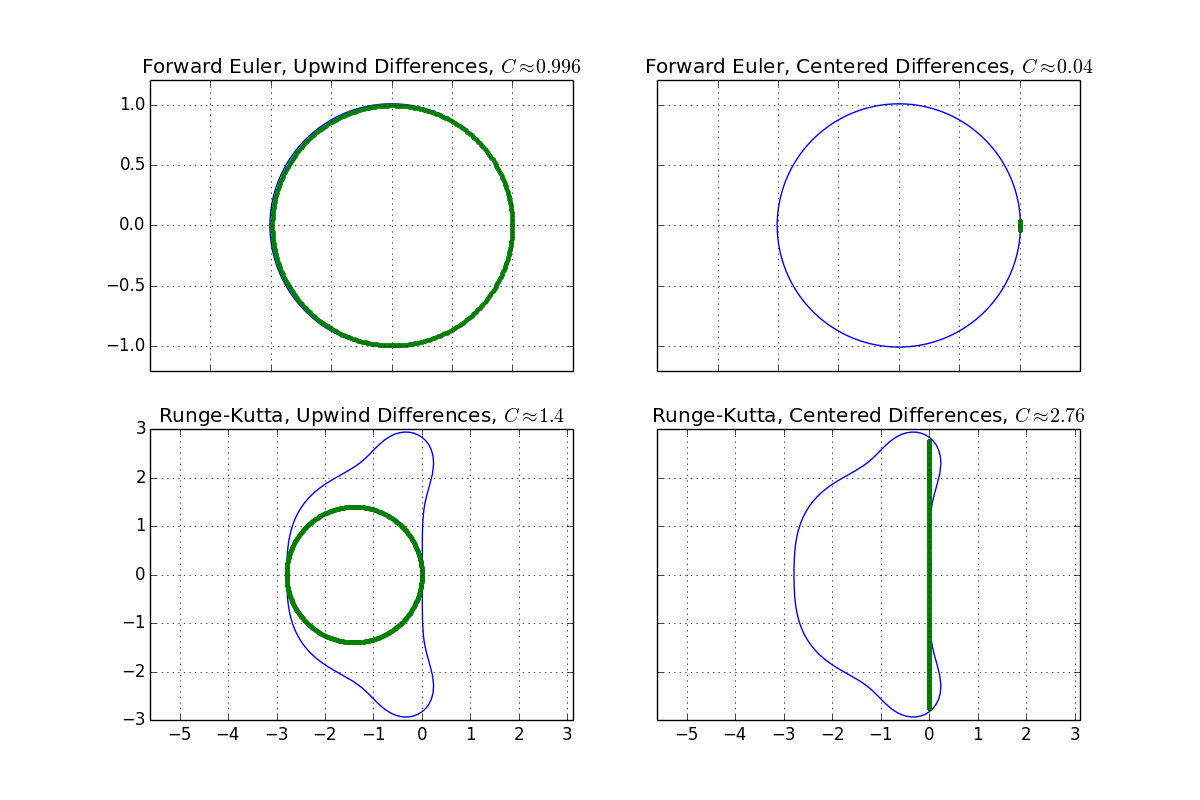
\includegraphics[scale=0.6]{stability_regions}
\end{figure}

When I actually run my solver with forward Euler and centered differences, it is ubstable for any $\Delta t$ I pick. This makes sense since the eigenvalues of the corresponding matrix are purely imaginary and the intersection of the stability region for Forward Euler's method with the imaginary axis is the origin, i.e. none of the eigenvalues except zero fall into the stability region.

\item[(b)] See \verb+pde.py+ for my code. Below are my plots for the three stable combinations for each of the three initial functions. In each plot, I only plotted the solution for the first two periods in time.

\begin{figure}[H]
  \centering
  \caption{Forward Euler method, upwind differences}
  \vspace{5 mm}
    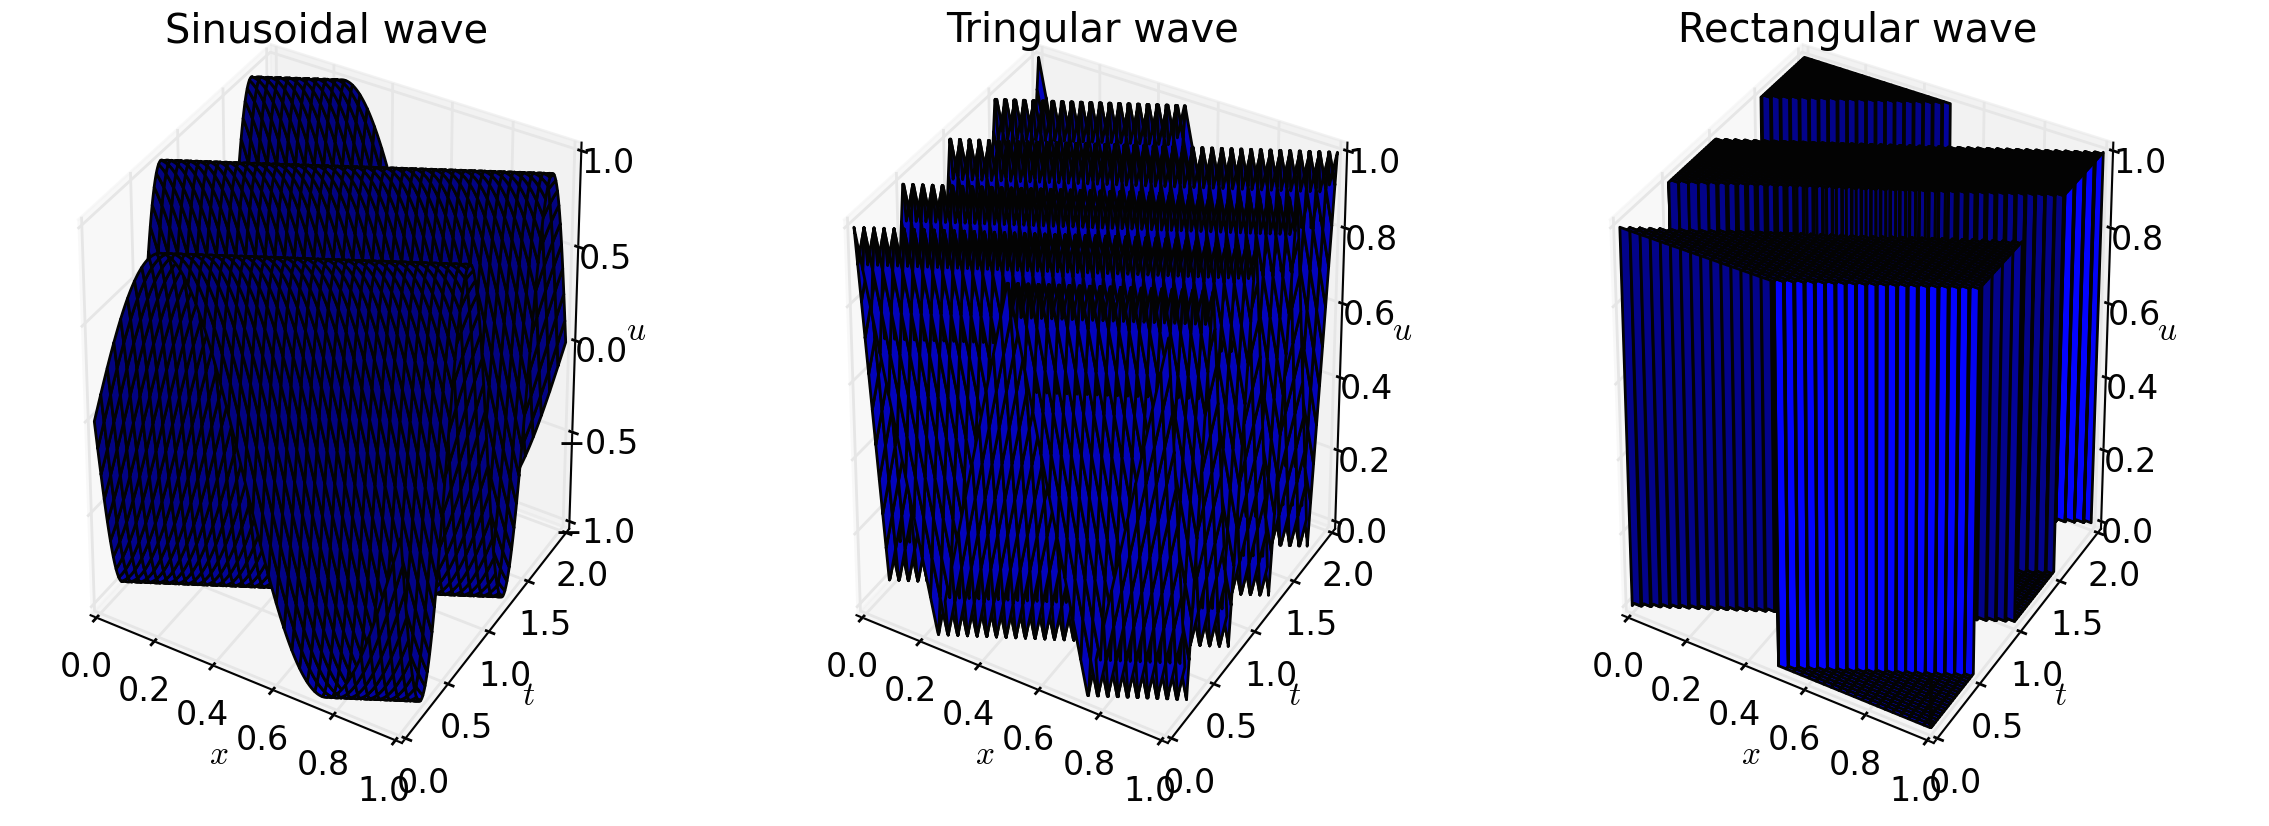
\includegraphics[scale=0.5]{pde_solution_combo1}
\end{figure}

\begin{figure}[H]
  \centering
  \caption{4th order Runge-Kutta method, upwind differences}
  \vspace{5 mm}
    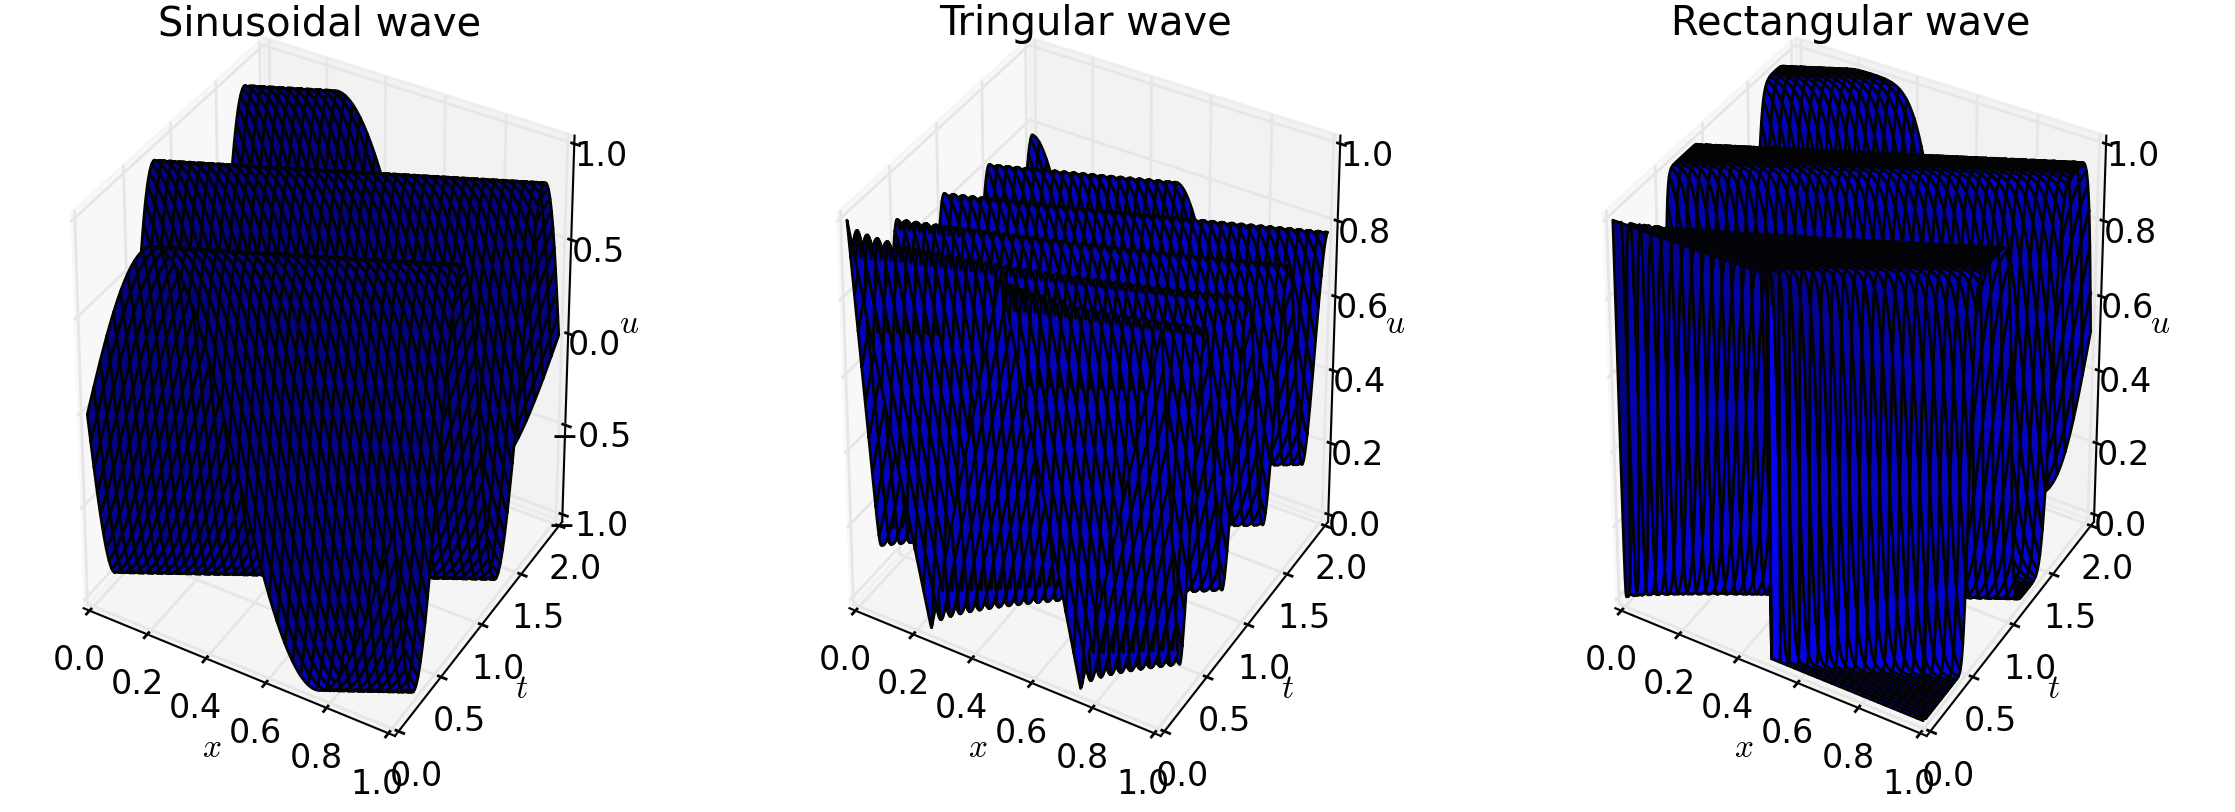
\includegraphics[scale=0.5]{pde_solution_combo2}
\end{figure}

\begin{figure}[H]
  \centering
   \caption{4th order Runge-Kutta method, centered differences}
   \vspace{5 mm}
    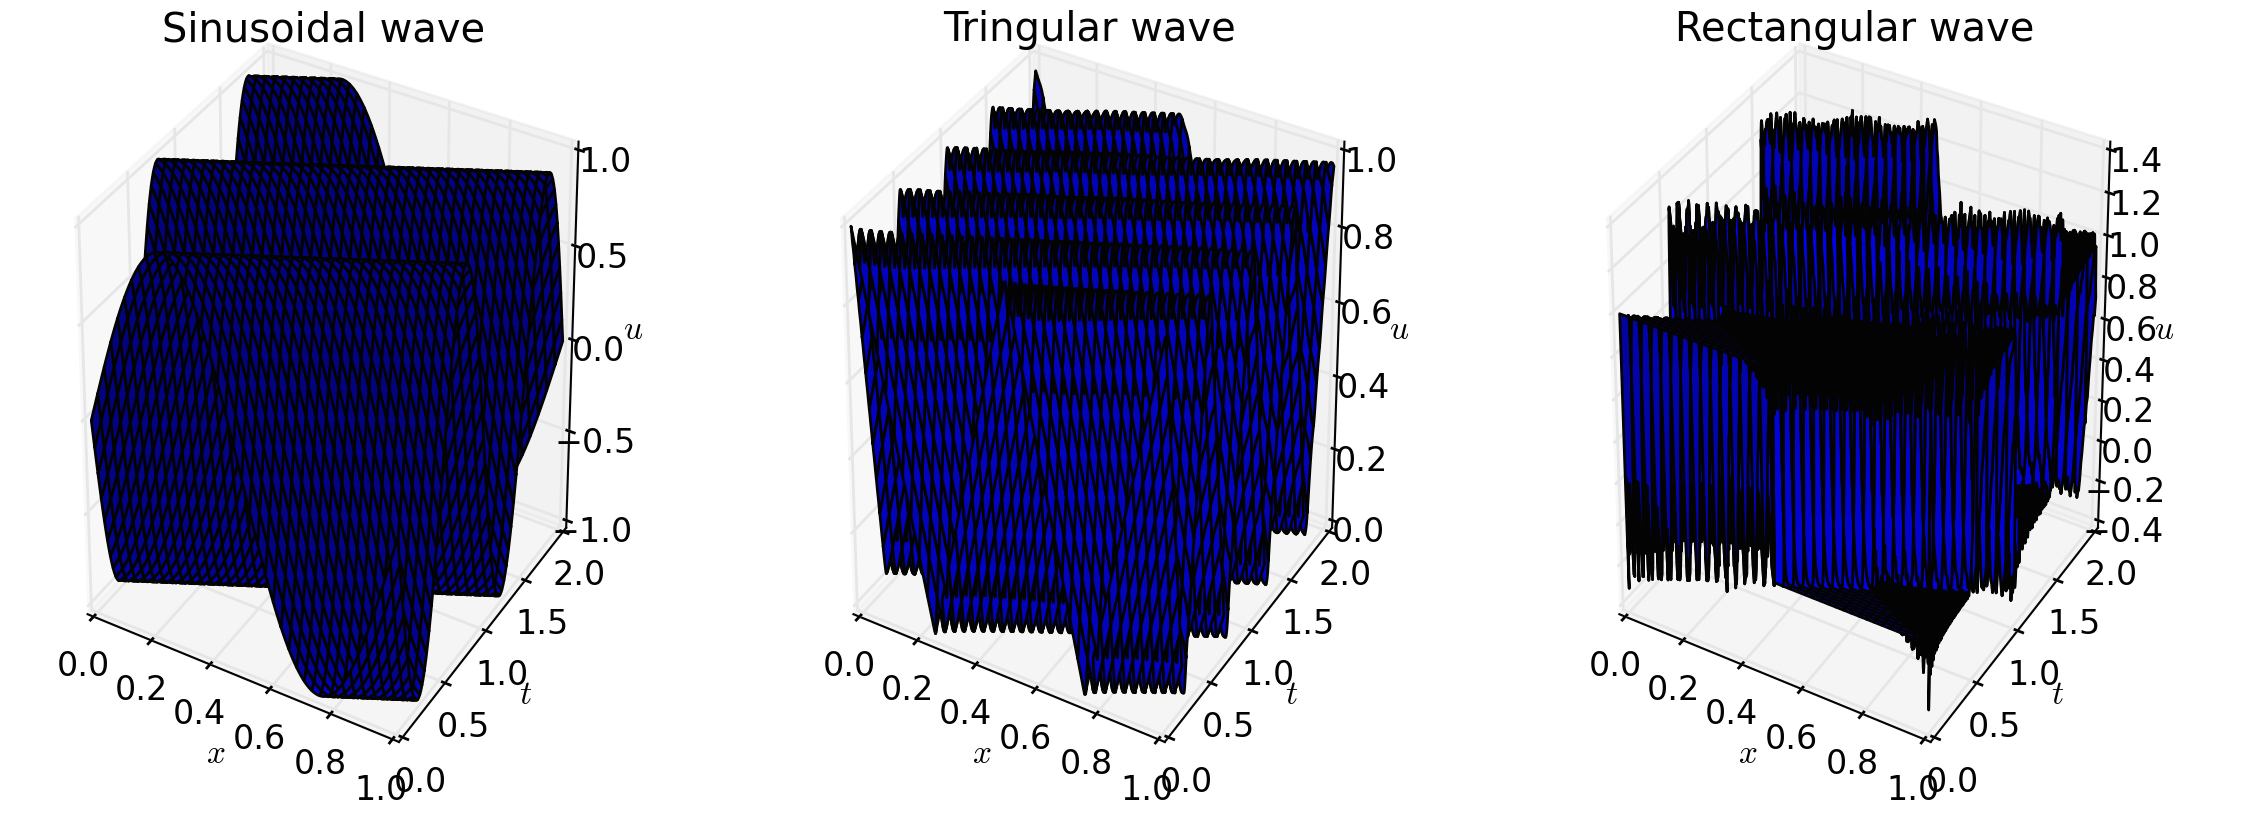
\includegraphics[scale=0.5]{pde_solution_combo3}
\end{figure}

For extra analysis of error propagation, I plotted the $ L^p, p = 1,2, \infty $ error of the approximate solutions over time $$\xi_p(u_{\Delta t}, t) = \left( \int_{0}^{1}| u_{\Delta t}(x,t) - u(x,t) |^p \, dx \right)^{1/p}, $$ where $ u_{\Delta t}(x,t) $ is the approximate solution and $  u(x,t)  $ is the exact solution, for all of the cases and methods. See my plots below. You can see that forward Euler's method with upwind differences and 4th order Runge-Cutta with centered differences are the best combinations and that forward Euler's method with centered differences is unstable. In each case, I let $ \Delta t = \Delta x $.

\begin{figure}[H]
  \centering
  \caption{$L^p$ error vs. time, Sinusoidal wave}
    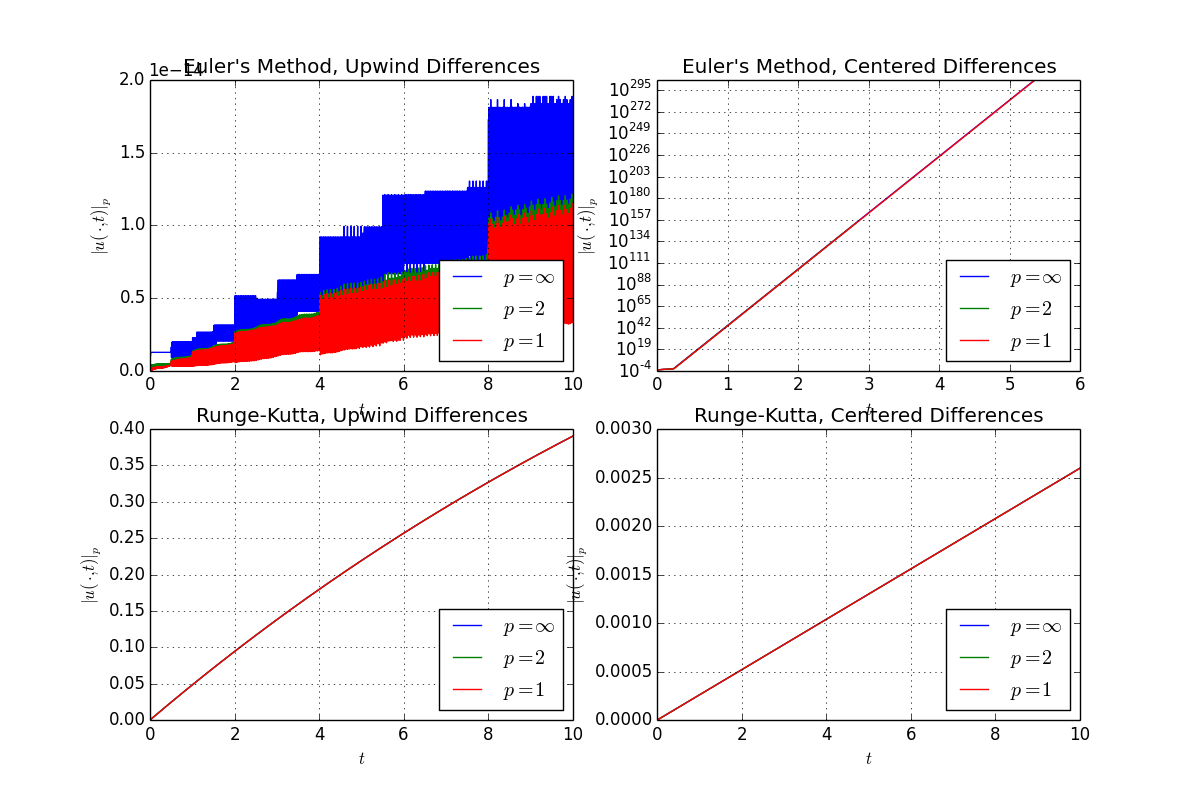
\includegraphics[scale=0.5]{pde_errs_case1}
\end{figure}

\begin{figure}[H]
  \centering
  \caption{$L^p$ error vs. time, Tringular wave}
    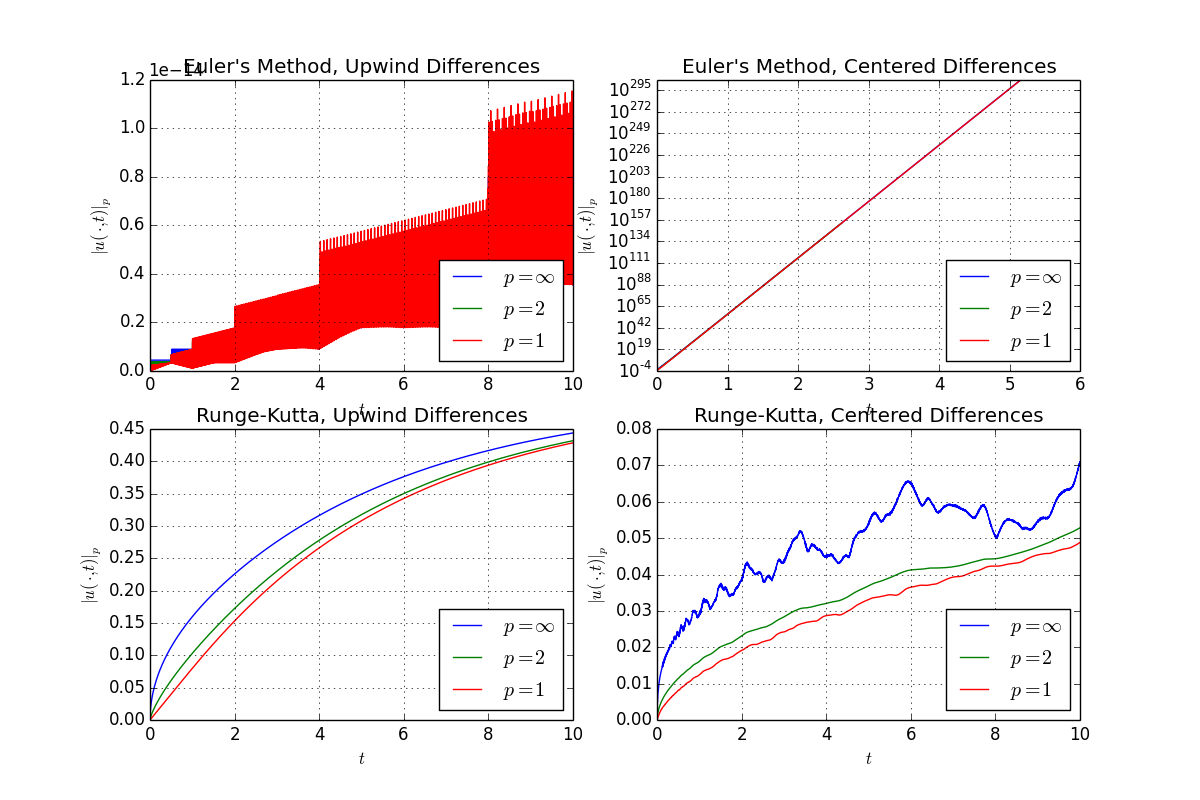
\includegraphics[scale=0.5]{pde_errs_case2}
\end{figure}

\begin{figure}[H]
  \centering
  \caption{$L^p$ error vs. time, Rectangular wave}
    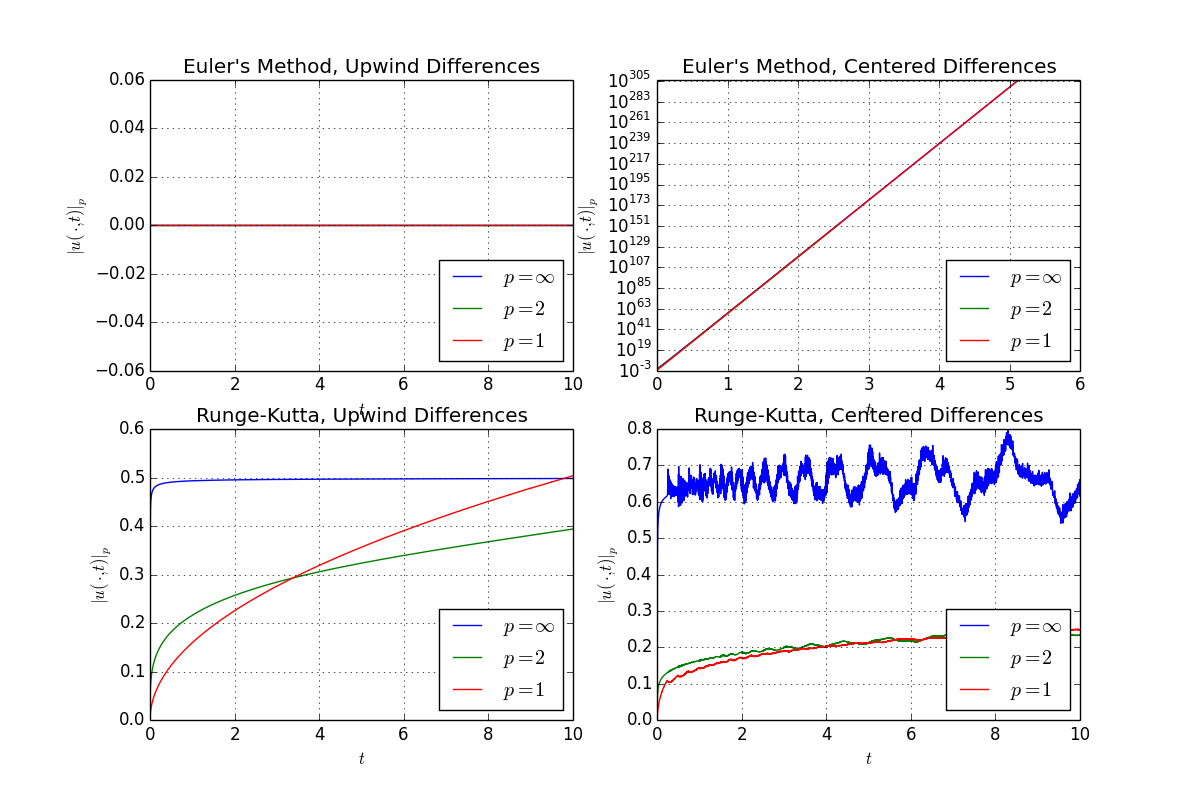
\includegraphics[scale=0.5]{pde_errs_case3}
\end{figure}

\end{itemize}

\end{document}

